\newif\ifnotes

% Uncomment either one to render the document with or without notes
%\notestrue
\notesfalse

% Adjust beamer template
\documentclass[aspectratio=169,xcolor=dvipsnames]{beamer}

\usetheme{Simple}

\setbeamertemplate{footline}[frame number]{} % Use frame numbers instead of page numbers
\ifnotes
    \setbeamertemplate{note page}[plain]
    \setbeameroption{show notes on second screen=bottom}
\fi

\usepackage{hyperref}
\usepackage{graphicx}
\usepackage{booktabs}

\usepackage[outputdir=build]{minted}

% Overwrite minted style
\setminted[Rust]{
    breaklines=true,
    escapeinside=''
}

\usemintedstyle{manni}

% Macro color for overwriting if the macro is not recognized
\definecolor{macro}{rgb}{0.80, 0.00, 1.00}

% Commands
\newcommand{\rust}[1]{\mintinline{rust}{#1}}
\newcommand{\nohighlight}[1]{\mintinline{TeX}{#1}}
\newcommand{\enote}[1]{
    \note{
        \textbf{Notes:}
        \begin{enumerate}
            #1
        \end{enumerate}
    }
}
\newcommand{\so}{$\rightarrow$ }
\newcommand{\br}{\vspace{\baselineskip}}

% !TeX root = ../main.tex
\title[Rust for Network Servers]{Rust for Network Servers}
\subtitle{Synchronous and asynchronous network communication}

\author[Simon Pannek] {Simon Pannek}
\institute[TUM]{
    Technical University of Munich \\
    Munich, Germany
    \vskip 3pt
}
\date{\today}


\begin{document}

% Title
\begin{frame}
    \titlepage
\end{frame}

% Slides

% Chapter 1 (Introduction)
% !TeX root = ../main.tex
\begin{frame}{Introduction}
    \center{Back in the 1960s the protocols for one of the first computer networks were developed.}
    \begin{figure}
        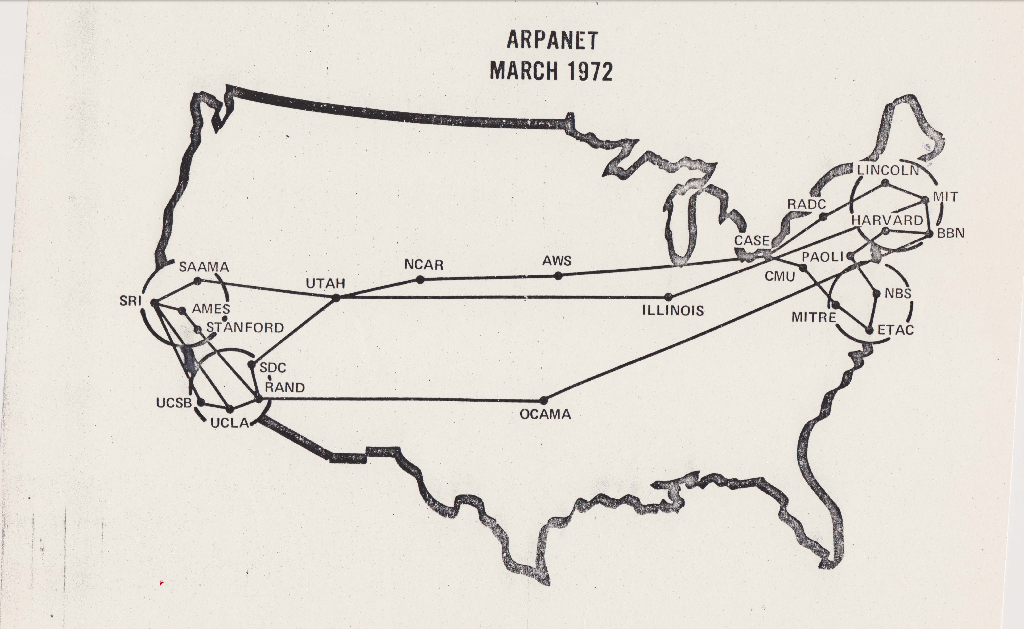
\includegraphics[width=0.5\linewidth]{images/arpanet_1972.png}
        \caption{Ferris the Crab \cite{arpanet}}
    \end{figure}

    \enote{
        \item Many modern devices used today are using the internet to communicate with each other
        \item A foundation for this can be found when looking at the ARPANET
        \item ARPANET: A packet-switching network deployed in the US
        \begin{enumerate}
            \item One of the first networks to implement the TCP/IP protocol suite
            \item Evolved into the Internet as we know it today
        \end{enumerate}
    }
\end{frame}

% !TeX root = ../main.tex
\begin{frame}{Introduction}
    \textbf{What happened until now?}
    \begin{enumerate}
        \item<1-> Additional security (encryption)
        \item<2-> Introduction of new protocols
        \item<3> A lot was standardized (IEEE standards, W3C, ...)
    \end{enumerate}
\end{frame}

% !TeX root = ../main.tex
\begin{frame}{Introduction}
    \Huge
    \centerline{What programming language to choose?}

    \enote{
        \item Standardization \so common used programming language usually support frequently deployed networking
        protocols
        \item Depends on the use case: Certain trade offs comparing different languages
        \item We are going to take a look at Rust and what it has to offer when it comes to running it as a backend of
        a network application
    }
\end{frame}


% !TeX root = ../main.tex
\begin{frame}[fragile]{Introduction}
    \begin{enumerate}
        \item[]<2> \Huge
        \centerline{Buffer Overflow Attacks}

        \item[]<1-> \Large
        \begin{minted}{C}
            void unsecure_function(void) {
                char buf[512];
                read_from_network(buf);

                ...
            }
        \end{minted}
    \end{enumerate}

    \enote{
        \item Let us take a step back: Currently, many networking libraries are written in C or C++
        \item What is the problem with this piece of code?
        \item Buffer overflow attacks (Small explanation what can happen)
        \item No guaranteed memory safety in C and C++
        \item Mistakes of a programmer are not checked by the compiler and fall back to some default action (UB \so
        corruption of memory)
        \item Problematic for network applications (many concurrent reads and writes to buffers)
    }
\end{frame}

% !TeX root = ../main.tex
\begin{frame}[fragile]{Introduction}
    \begin{enumerate}
        \item[]<2> \Huge
        \centerline{Interpreted languages}

        \item[]<1-> \Large
        \begin{minted}{Python}
            def more_secure_function(socket):
                buf = socket.recv(512)
    
                ...
        \end{minted}
    \end{enumerate}

    \enote{
        \item Simplified example \so Depends on the actual use case and implementation whether something can be
        considered secure
        \item Interpreted languages like Python as a solution (background checks for undefined behavior for almost
        everything)
        \item Scripting languages allow fast prototyping
        \item Trade off of interpreted languages: Slower performanced compared to executing compiled binary files
        (Instructions first have to get translated by the interpreter)
        \item They do not run natively on the computer \so you first have to install the interpreter
    }
\end{frame}

% !TeX root = ../main.tex
\begin{frame}{Introduction}
    \Huge
    \centerline{Rust as a solution?}

    \br

    \begin{figure}
        
\includegraphics[width=0.3\linewidth]{images/ferris.png}
        \caption{Ferris the Crab \cite{ferris}}
    \end{figure}

    \enote{
        \item Rust can be considered "the best of both worlds":
        \begin{enumerate}
            \item Compiled language with a compiler guaranteeing memory- and thread-safety
            \item Fast speed of compiled languages and prevents most of the vulnerabilities mentioned before through
                  its compiler checks
            \item Network operations are prune to failure \so unsafe calls can be wrapped into enums of the type
                  \rust{std::result::Result}
            \item Package manager Cargo
        \end{enumerate}
        \item Let us first take a look how to implement basic TCP and UDP communication in Rust
    }
\end{frame}



% Chapter 2 (Networking in Rust)
% !TeX root = ../main.tex
\begin{frame}{Networking in Rust}
    \Huge
    \centerline{Ownership, borrowing, and lifetimes}

    \pause

    \br

    \Large
    \centerline{\so No dangling references, illegal memory access, and memory leaks}

    \pause

    \br

    \small
    \centerline{(Except if you are explicitly working with \rust{unsafe} code)}

    \enote{
        \item Ownership, borrowing and lifetimes play an important role in networking code
        \item Ownership:
        \begin{enumerate}
            \item A part of the code can own a piece of memory
            \item Function is called with an owned value \so the piece of memory gets moved into that function
        \end{enumerate}
        \item Borrowing:
        \begin{enumerate}
            \item No complete access is needed \so a reference can be borrowed
            \item There are also mutable reference: Only one is allowed at the same time
            \item Useful whne working with network applications (prevents the occurence of data races if a thread tires
                  to read or write to a buffer while another thread is already writing to it)
            \item We are not going to take a look at \rust{std::sync::Arc}
        \end{enumerate}
        \item Lifetimes:
        \begin{enumerate}
            \item Lifetime determined by the code block it was created \so variable gets out of scope \so the
                  corresponding piece of memory is freed
            \item If a value gets moved into another function, its lifetime changes with it
        \end{enumerate}
    }
\end{frame}


% !TeX root = ../main.tex
\begin{frame}{Networking in Rust}
    \textbf{The Transmission Control Protocol (TCP)}

    \begin{itemize}
        \item<2-> Active connection between two systems
        \item<3-> Can be used to send a continous stream of octets to another host
        \item<4-> A sequence number is assigned to each octet in order to confirm it was received
        \item<5> If no acknowledgment (ACK) was received, the data is sent again
    \end{itemize}

    \enote{
        \item TCP is used for reliable inter-process communication between two systems connected through a network
        \item The sequence number can also be used to eliminate duplicates
        \item \rust{std::net} module includes networking functions for TCP
    }
\end{frame}

% !TeX root = ../main.tex
\begin{frame}[fragile]{Networking in Rust}
    \begin{block}{TCP client handling}
        \begin{overprint}
            \onslide<1>
            \begin{minted}{Rust}
            let mut reader = BufReader::new(&stream);
            
            loop {
                let mut buf = String::new();
            
                match reader.read_line(&mut buf) {
                    '\Large{...}'
                }
            }
            \end{minted}

            \onslide<2>
            \begin{minted}{Rust}
            match reader.read_line(&mut buf) {
                Ok(0) => break,
                Ok(_) => print!("{}", buf),
                Err(e) => {
                    eprintln!("{}", e);
                    stream.shutdown(Both)?;
                    break;
                }
            }
            \end{minted}
        \end{overprint}
    \end{block}
\end{frame}

% !TeX root = ../main.tex
\begin{frame}[fragile]{Networking in Rust}

    \begin{block}{TCP listener}
        \begin{minted}{Rust}
            let listener = TcpListener::bind(ADDRESS)
                .expect("Bind to address");
            
            for stream in listener.incoming() {
                if let Ok(stream) = stream {
                    handle_client(stream)
                        .expect("Handle client");
                }
            }
        \end{minted}
    \end{block}
\end{frame}

% !TeX root = ../main.tex
\begin{frame}[fragile]{Networking in Rust}

    \begin{block}{TCP client}
        \begin{overprint}
            \onslide<1>
            \begin{minted}{Rust}
            let mut stream = TcpStream::connect(ADDRESS)?;

            loop {
                let mut buf = String::new();
            
                match stdin().read_line(&mut buf) {
                    '\Large{...}'
                }
            }
            \end{minted}

            \onslide<2>
            \begin{minted}{Rust}
                match stdin().read_line(&mut buf) {
                    Ok(_) => {
                        '\Large{...}'
                    }
                    Err(e) => {
                        eprintln!("{}", e);
                        stream.shutdown(Both)?;
                        break;
                    }
                }
            \end{minted}

            \onslide<3>
            \begin{minted}{Rust}
                Ok(_) => {
                    let bytes = buf.as_bytes();
        
                    stream
                        .write_all(bytes)
                        .expect("Writing");
                }
            \end{minted}
        \end{overprint}
    \end{block}
\end{frame}


% !TeX root = ../main.tex
\begin{frame}{Networking in Rust}
    \textbf{The User Datagram Protocol (UDP)}
    \begin{itemize}
        \item<2-> Commonly used if you do not need reliable delivery of streams
        \item<3-> Tries to send messages to other programs with a minimal amount of protocol mechanism
        \item<4-> No protection against package duplication
        \item<5> No checks whether the data sent has arrived and if it did in what order
    \end{itemize}

    \enote{
        \item UDP is less reliable than the Transmission Control Protocol
        \item No need to listen for new hosts or actively establish a connection
        \item Typical example: Media streaming (package loss is acceptable)
    }
\end{frame}

% !TeX root = ../main.tex
\begin{frame}[fragile]{Networking in Rust}

    \begin{block}{UDP receiver}
        \begin{overprint}
            \onslide<1>
            \begin{minted}{Rust}
            let socket = UdpSocket::bind(ADDRESS)?;

            loop {
                let mut buf = [0u8; 1500];
            
                match socket.recv_from(&mut buf) {
                    '\Large{...}'
                }
            }
            \end{minted}

            \onslide<2>
            \begin{minted}{Rust}
            match socket.recv_from(&mut buf) {
                Ok(_) => {
                    let msg = from_utf8(&buf)
                        .expect("Convert data");
        
                    print!("{}", msg);
                }
                Err(e) => {
                    eprintln!("{}", e);
                    break;
                }
            }
            \end{minted}
        \end{overprint}
    \end{block}

    \enote{
        \item Why is the buffer size 1500? (Maximum Transmission Unit)
        \item Why is a buffer needed at all? (\rust{std::net::UdpSocket} does not implement the trait
        \rust{std::io::Read})
    }
\end{frame}

% !TeX root = ../main.tex
\begin{frame}[fragile]{Networking in Rust}
    \begin{block}{UDP sender}
        \begin{overprint}
            \onslide<1>
            \begin{minted}{Rust}
            let socket = UdpSocket::bind("0.0.0.0:0")?;

            loop {
                let mut buf = String::new();
            
                match stdin().read_line(&mut buf) {
                    '\Large{...}'
                }
            }
            \end{minted}

            \onslide<2>
            \begin{minted}{Rust}
            match stdin().read_line(&mut buf) {
                Ok(_) => {
                    let bytes = buf.as_bytes();
        
                    socket
                        .send_to(bytes, ADDRESS)
                        .expect("Sending");
                }
                Err(e) => {
                    eprintln!("{}", e);
                    break;
                }
            }
            \end{minted}
        \end{overprint}
    \end{block}
\end{frame}



% Chapter 3 (Asynchronous Networking using Tokio)
% !TeX root = ../main.tex
\begin{frame}{Asynchronous Networking in Rust}
    \begin{table}
        \begin{tabular}{l l}
            \toprule
            \textbf{Sequential programming}          & \textbf{Asynchronous programming}       \\
            \midrule
            - Blocking functions                     & - Non blocking functions                \\
            - Result is returned immediately         & - Result is wrapped into futures        \\
            - A new thread is required for each task & - A scheduler dynamically assigns tasks \\
            which is not finished yet                & to a limited amount of threads          \\
            \bottomrule
        \end{tabular}
        \caption{Comparison between sequential and asynchronous programming}
    \end{table}

    \enote{
        \item Previous examples: Current thread was blocked when waiting for new connections/incoming messages
        \item Sequential programming: Scheduler swaps out the waiting task
    }
\end{frame}

% !TeX root = ../main.tex
\begin{frame}{Asynchronous Networking in Rust}
    \textbf{The Tokio crate}

    \begin{itemize}
        \item<2-> Tokio is a runtime for writing reliable network applications \cite{tokio-doc}
        \item<3-> Tokio consists of three major parts:
        \begin{enumerate}
            \item<4-> I/O event loop
            \item<5-> Timer
            \item<6> Scheduler
        \end{enumerate}
    \end{itemize}

    \enote{
        \item Easily imported and managed via Cargo
        \item Includes feature flags \so specify which parts of the library should be included
        \item Parts of tokio:
        \begin{enumerate}
            \item I/O event loop: Handles I/O events and dispatches them to the tasks waiting for them
            \item Timer: Runs tasks after a certain period of time
            \item Scheduler: Executes the tasks on the different threads
        \end{enumerate}
        \item Enables the use of \rust{async}, \rust{await} and other features of asynchronous Rust
        \item \rust{tokio::net} includes networking functions similar to \rust{std::net}
    }
\end{frame}

% !TeX root = ../main.tex
\begin{frame}[fragile]{Asynchronous Networking in Rust}
    \begin{block}{Future demonstration}
        \begin{overprint}
            \onslide<1>
            \begin{minted}{Rust}
            async fn async_function() {
                println!("Started task1");
                sleep(Duration::from_secs(5))
                    .await;
                println!("Finished task1");
            }
            \end{minted}

            \onslide<2>
            \begin{minted}{Rust}
            #[tokio::main]
            async fn main() {
                let future1 = async_function();

                let future2 = async {
                    println!("Started task2");
                    sleep(Duration::from_secs(3))
                        .await;
                    println!("Finished task2");
                };

                '\textcolor{macro}{join!}'(future1, future2);
            }
            \end{minted}
        \end{overprint}
    \end{block}

    \enote{
        \item Complete asynchronous function declaration vs. \rust{async} block
        \item Execution in blocking environment:
        \begin{enumerate}
            \item Started task1
            \item Finished task1
            \item Started task2
            \item Finished task2
        \end{enumerate}
        \item Execution in non-blocking environment:
        \begin{enumerate}
            \item Started task1
            \item Started task2
            \item Finished task2
            \item Finished task1
        \end{enumerate}
    }
\end{frame}


% !TeX root = ../main.tex
\begin{frame}[fragile]{Asynchronous Networking in Rust}
    \begin{block}{Asynchronous TCP client handling}
        \begin{overprint}
            \onslide<1>
            \begin{minted}{Rust}
            tokio::spawn(async move {
                let mut reader = BufReader::new(&mut stream);
            
                loop {
                    let mut buf = String::new();
            
                    match reader.read_line(&mut buf).await {
                        '\Large{...}'
                    }
                }
            
                Ok::<(), Error>(())
            });
            \end{minted}

            \onslide<2>
            \begin{minted}{Rust}
            match reader.read_line(&mut buf).await {
                Ok(0) => break,
                Ok(_) => print!("{}", buf),
                Err(e) => {
                    eprintln!("{}", e);
                    stream
                        .shutdown().await?;
                    break;
                }
            }
            \end{minted}
        \end{overprint}
    \end{block}

    \enote{
        \item \rust{async move} \so the asynchronous block will take the ownership of all variables referenced within it
        \item Without this all variables would be bound to the scope of the code surrounding it
        \item Full ownership of \rust{stream} is required
    }
\end{frame}

% !TeX root = ../main.tex
\begin{frame}[fragile]{Asynchronous TCP client handling}
    \begin{block}{Asynchronous TCP listener}
        \begin{minted}{Rust}
            let listener = TcpListener::bind(ADDRESS).await?;

            loop {
                let (stream, _) = listener.accept().await?;

                handle_client(stream);
            }
        \end{minted}
    \end{block}
\end{frame}

% !TeX root = ../main.tex
\begin{frame}[fragile]{Asynchronous Networking in Rust}
    \begin{block}{Asynchronous TCP client}
        \begin{overprint}
            \onslide<1>
            \begin{minted}{Rust}
            let mut stream = TcpStream::connect(ADDRESS).await?;

            let mut reader = BufReader::new(stdin());
            
            loop {
                let mut buf = String::new();
            
                match reader.read_line(&mut buf).await {
                    '\Large{...}'
                }
            }
            \end{minted}

            \onslide<2>
            \begin{minted}{Rust}
            match reader.read_line(&mut buf).await {
                Ok(_) => {
                    '\Large{...}'
                }
                Err(e) => {
                    eprintln!("{}", e);
                    stream.shutdown().await?;
                    break;
                }
            }
            \end{minted}

            \onslide<3>
            \begin{minted}{Rust}
            Ok(_) => {
                let bytes = buf.as_bytes();
    
                stream
                    .write_all(bytes)
                    .await?;
            }
            \end{minted}
        \end{overprint}
    \end{block}
\end{frame}


% !TeX root = ../main.tex
\begin{frame}{Asynchronous Networking in Rust}
    \Large
    \centerline{What about Asynchronous UDP communication?}

    \enote{
        \item Tokio offers \rust{tokio::net::UdpSocket} \so works similar to \rust{std::net::UdpSocket}
        \item Porting the synchronous UDP implementation to an asynchronous one works similarly to the TCP client
        \item UDP does not implement actual connections \so waiting for new connections is non blocking anyway
        \item The advantage of connecting to multiple clients for the asynchronous TCP client is not given for UDP
        \item Client should also send messages? \rust{std::sync::Arc} could be used \so shared ownership to the socket
        (no mutable reference needed for \rust{send_to} and \rust{recv_from})
    }
\end{frame}


% !TeX root = ../main.tex
\begin{frame}{Asynchronous Networking in Rust}
    \Huge
    \centerline{Network Client Showcase}
\end{frame}



% Chapter 4 (Application Layer communication)
% !TeX root = ../main.tex
\begin{frame}{Application Layer communication}
    \center{
        \begin{minipage}{4cm}
            \begin{table}
                \begin{tabular}{l}
                    \toprule
                    \textbf{OSI layers}           \\
                    \midrule
                    \begin{overprint}
                        \onslide<1>
                        Application Layer
                        \onslide<2>
                        \textbf{Application Layer}
                    \end{overprint} \\
                    Presentation Layer            \\
                    Session Layer                 \\
                    \begin{overprint}
                        \onslide<1>
                        \textbf{Transport Layer}
                        \onslide<2>
                        Transport Layer
                    \end{overprint} \\
                    Network Layer                 \\
                    Data Link Layer               \\
                    Physical Layer                \\
                    \bottomrule
                \end{tabular}
            \end{table}
        \end{minipage}
    }

    \enote{
        \item Layers (just in case):
        \begin{enumerate}
            \item Application Layer: Network Process to Application
            \item Presentation Layer: Data representation and Encryption
            \item Session Layer: Interhost communication
            \item Transport Layer: End-to-End connections
            \item Network Layer: Path Determination and logical addressing
            \item Data Link Layer: Physical addressing
            \item Physical Layer: Media, signal and binary transmission
        \end{enumerate}
        \item Showcase how Tokio can be used together with higher level protocols
        \item Hypertext Transfer Protocol (HTTP) for data transmission for the World Wide Web (usually based on TCP)
    }
\end{frame}

% !TeX root = ../main.tex
\begin{frame}[fragile]{Application Layer communication}
    \begin{block}{Data struct}
        \begin{minted}{Rust}
            #[derive(Serialize, Deserialize, Debug)]
            struct Data {
                number: u32,
                boolean: bool,
            }
        \end{minted}
    \end{block}

    \enote{
        \item Crate "Serde" allows for simple serialize and deserialize implementation
        \item Convert data instances from and to JSON (JavaScript Object Notation)
        \item Required to send objects over HTML
    }
\end{frame}

% !TeX root = ../main.tex
\begin{frame}[fragile]{Application Layer communication}
    \begin{block}{Warp HTTP server}
        \begin{minted}{Rust}
            let filter = warp::'\textcolor{macro}{path!}'("data")
                .and(warp::post())
                .and(warp::body::json())
                .map(|data: Data| format!("Received: {:?}", data));

            warp::serve(filter).run(ADDRESS).await;
        \end{minted}
    \end{block}

    \enote{
        \item Crate "Warp" is a simple web framework built on another create called "Hyper"
        \item Works together with Tokio
        \item \rust{warp::Filter}:
        \begin{enumerate}
            \item Extracts data from a request, handles the data and sends a response back to the sender of the request
            \item \rust{and}-method: Chains together two filters
            \item \rust{map}-method: Takes a function as an argument, receives the extracted data and maps it to
                  another value
        \end{enumerate}
    }
\end{frame}

% !TeX root = ../main.tex
\begin{frame}[fragile]{Application Layer communication}
    \begin{block}{Reqwest HTTP client}
        \begin{minted}{Rust}
            let client = reqwest::Client::new();

            let response = client
                .post(URL)
                .json(&Data {
                    number: 5,
                    boolean: true,
                })
                .send()
                .await
                .expect("Sending request");

            println!("{}", response.text().await.expect("Get text"));
        \end{minted}
    \end{block}

    \enote{
        \item Crate "Reqwest" enables sending simple HTTP requests
        \item Requires some kind of runtime like Tokio
    }
\end{frame}

% !TeX root = ../main.tex
\begin{frame}[fragile]{Application Layer communication}
    \begin{alertblock}{Client response}
        \begin{minted}{TeX}
            Received: Data { number: 5, boolean: true }
        \end{minted}
    \end{alertblock}
\end{frame}



% Chapter 5 (Conclusion)
% !TeX root = ../main.tex
\begin{frame}{Conclusion}
    \Large
    \centerline{Rust is a very powerful language for writing network applications}

    \enote{
        \item Often important to deploy a secure and efficient language as a backend
        \item Underlying services can be considered the bottleneck most of the times
        \item Slowing down or outages should be avoided
        \item Security vulnerabilites can cause interruption of service or accidental disclosure of sensible user data
        \item Rust's compile time checks can avoid many common security issues
        \item Shifting checks into the process of compiling the code removes checking at runtime, making executables
        even faster
    }
\end{frame}

% !TeX root = ../main.tex
\begin{frame}{Conclusion}
    \begin{figure}
        \huge
        \centerline{Are there any questions?}

        \br

        
\includegraphics[width=0.4\linewidth]{images/ferris.png}
        \caption{Ferris the Crab \cite{ferris}}
    \end{figure}
\end{frame}



% References
\begin{frame}{References}
    \begin{columns}[c]

        % Left column
        \column{.5\textwidth}

        \footnotesize {
            \begin{thebibliography}{9}

                \bibitem[1]{arpanet} UCLA and BBN (1972) [1]
                \newblock The map of ARPANET in March 1972.
                \newblock \url{https://commons.wikimedia.org/wiki/File:Arpanet_1972_Map.png}

                \bibitem[2]{tokio-doc} Docs.rs/tokio [2]
                \newblock Tokio crate documentation.
                \newblock \url{https://docs.rs/tokio/1.6.1/tokio/}

                \bibitem[3]{ferris} Rustacean.net [3]
                \newblock Ferris the Crab.
                \newblock \url{https://rustacean.net/assets/rustacean-flat-happy.png}

            \end{thebibliography}
        }

        % Right column
        \column{.5\textwidth}

    \end{columns}
\end{frame}


\end{document}
